% 2007 年陕西卷理科第 19 题：底面为直角梯形的四棱锥 P-ABCD，PA⊥底面。
%   AD∥BC，∠ABC=90°，PA=3，AD=2，AB=2√3，BC=6；E 为 AC 与 BD 的交点。
% 来源 PDF：gaokaomath-src/普通高考/2007/2007陕西理.pdf
% SHA-256：95abaa3050f33e9b9587ad186af8f173fbf40c31ebe3f2be710bbae607ed0ecb
% 原页：2007陕西理.pdf 第 2 页（A3 三栏）第 1 栏，书页码 402。
% 重绘依据：按原页底面梯形、P 的位置与 E 点重绘。
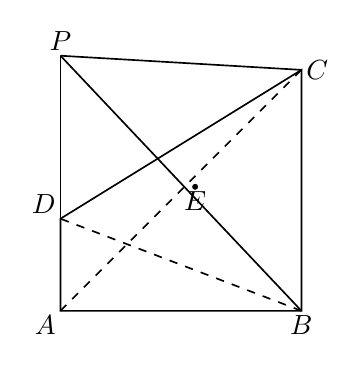
\begin{tikzpicture}[scale=0.9, semithick,
  every node/.style={inner sep=1.5pt}]
  \coordinate (A) at (0,0);
  \coordinate (B) at (3.4,0);
  \coordinate (C) at (3.4,3.4);
  \coordinate (D) at (0,1.3);
  \coordinate (P) at (0,3.6);
  \coordinate (E) at (1.9,1.75);

  \draw (A) -- (B) -- (C) -- (D) -- cycle;
  \draw (P) -- (A);
  \draw (P) -- (B);
  \draw (P) -- (C);
  \draw (P) -- (D);
  \draw[dashed] (A) -- (C);
  \draw[dashed] (B) -- (D);
  \fill (E) circle (1.2pt);

  \node[below left] at (A) {$A$};
  \node[below] at (B) {$B$};
  \node[right] at (C) {$C$};
  \node[above left] at (D) {$D$};
  \node[above] at (P) {$P$};
  \node[below] at (E) {$E$};
\end{tikzpicture}
